% 首页信息自动生成

\section{数学符号}
\begin{table}[H]
    \centering
    \begin{tabular}{l >{$\displaystyle}c<{$} >{\ttfamily}c}
        \toprule
        名称 & \multicolumn{1}{c}{样式} & \multicolumn{1}{c}{命令}\\
        \midrule
        绝对值 & \abs{x} & \textbackslash abs\{x\}\\
        范数 & \norm{v} & \textbackslash norm\{v\}\\
        期望值 & \Ex{X} & \textbackslash Ex\{X\}\\
        条件期望 & \Ex[Y]{X} & \textbackslash Ex[Y]\{X\}\\
        概率 & \Pr{A} & \textbackslash Pr\{A\}\\
        条件概率 & \Pr[B]{A} & \textbackslash Pr[B]\{A\}\\
        协方差 & \Cov{X}{Y} & \textbackslash Cov\{X\}\{Y\}\\
        方差 & \Var{X} & \textbackslash Var\{X\}\\
        极小值 & \argmin[x]{f(x)} & \textbackslash argmin[x]\{f(x)\}\\
        极大值 & \argmax[x]{g(x)} & \textbackslash argmax[x]\{g(x)\}\\
        超长符号 & \longstack{~}{BCDEFGHIJKLM} & \textbackslash longstack\{\textasciitilde\}\{BCDEFGHIJKLM\}\\
        \bottomrule
    \end{tabular}
\end{table}

\section{标记}
\begin{table}[H]
    \centering
    \begin{tabular}{l >{$\displaystyle}c<{$} >{\ttfamily}c}
    \toprule
    名称 & \multicolumn{1}{c}{样式} & \multicolumn{1}{c}{命令}\\
    \midrule
    下划线 & \muline{xxxx} & \textbackslash muline\{xxxx\}\\
    双下划线 & \muuline{xxxx} & \textbackslash muuline\{xxxx\}\\
    波浪下划线 & \muwave{xxxx} & \textbackslash muwave\{xxxx\}\\
    删除线 & \msout{xxxx} & \textbackslash msout\{xxxx\}\\
    多条斜线删除标记 & \mxout{xxxx} & \textbackslash mxout\{xxxx\}\\
    虚下划线 & \mdashuline{xxxx} & \textbackslash mdashuline\{xxxx\}\\
    点状虚下划线 & \mdotuline{xxxx} & \textbackslash mdotuline\{xxxx\}\\
    \bottomrule
    \end{tabular}
\end{table}

\section{图表}
\begin{figure}[H]
\centering
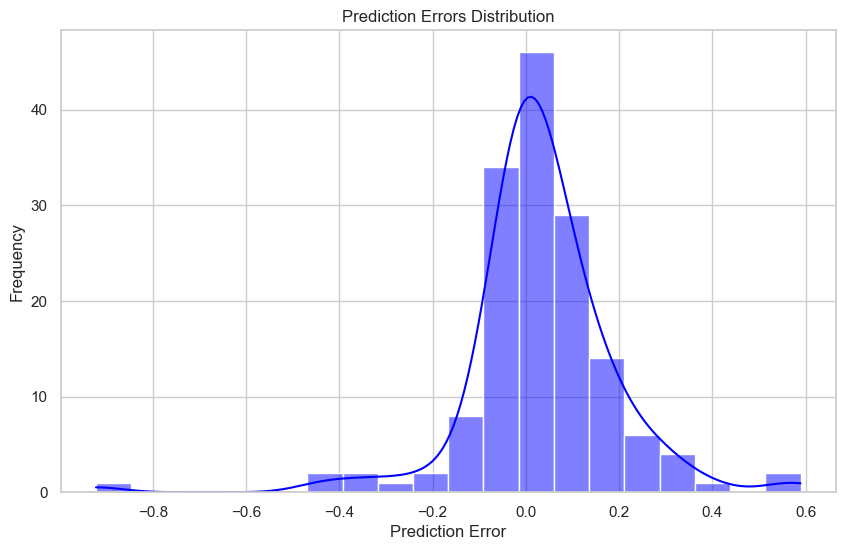
\includegraphics[width=0.3\textwidth]{test.png}
\caption{图片}
\label{fig:demo}
\end{figure}

\begin{table}[H]
\centering
\caption{表格}
\label{tab:demo}
\begin{tabular}{ll}
\toprule
项目 & 值 \\
\midrule
\subrow{一级条目} & 100 \\
\subrow{二级条目} & 200 \\
\bottomrule
\end{tabular}
\end{table}

图表引用:如\figref{fig:demo}所示,\tabref{tab:demo}展示了数据。

\section{代码}
\begin{itemize}
    \item 行内代码:\cmd{git commit -m "test"}
    \item 代码块:
    \begin{lst}[%
        language=python,
        displayName=PYTHON]
print("Hello World!")  # 简单输出
for i in range(10):
    !*\color{red}print(i)*!  # 带颜色逃逸
    \end{lst}
\end{itemize}

\section{题解环境}
\begin{prob}[难度系数]
这是一个多部分题目
\end{prob}
\begin{subsol}
\item 第一部分解:
\[ \int_0^1 x^2 dx = \frac{1}{3} \]
\item 第二部分解:
\begin{align*}
\Cov{X}{Y} &= \Ex{XY} - \Ex{X}\Ex{Y} \\
&= 0.5 - 0.2 \times 0.3 = 0.44
\end{align*}
\end{subsol}

\begin{prob}
证明勾股定理
\end{prob}
\begin{pf}
设直角三角形三边为$a,b,c$,则:
\[ a^2 + b^2 = c^2 \]
证毕。
\end{pf}

\section{化学式}
\chemfig{H_3C-[:30](-[:-90]OH)-[:-30]O-[:30]H} % 葡萄糖

\ce{CO2 + C -> 2 CO} % 化学反应式

\chemfig{*6((=O)-N(-CH_3)-(*5(=O)-N(-CH_3)-))} % 咖啡因

\ce{H2O} % 水分子

\chemfig{C(-[2]H)(-[6]H)(-[4]H)} % 甲烷

\ce{Zn^2+ + 2OH^- -> Zn(OH)2 v} % 沉淀反应

\chemfig{*6(=-N(-CH_3)-(*5(=O)-N(-CH_3)-))} % 尼古丁

\section{特殊功能}
跨行超链接:\url{https://www.thisisaverylooooooooooooooooooooooooooooooooooooooooooooooooooooooooooooooooooooooooooooooooooooooooooooooooooooooooooongurl.com/example/page?query=longurl}

\entertwocolumn
\section{临时双栏}
\lipsum[1]
\exittwocolumn

参考文献:引用文献\parencite{chen2016xgboost}
